\chapter{Implementation}
\label{chap:impl}
\chaptermark{Implementation}

This chapter describes what was built: signing in and how sessions are handled, what each user may do and how that is enforced, how their actions are recorded, and the security of the software the system runs on.

\section{Identity and Access Management}
\label{sec:impl-iam}

\subsection{Sign-in and Session Handling}

Users sign in through Keycloak, an identity provider running on the hospital's own servers, using OpenID Connect, a standard way for two systems to agree who someone is. The application never sees a password. It sends the user to Keycloak, and Keycloak sends back a token saying who they are and what role they hold. Password rules, account lockout, and the accounts themselves all live in Keycloak.

Roles are held in Keycloak and nowhere else. The application reads the role from the token and keeps no copy of its own. That is why there is no screen for editing permissions: to change what someone may do, an administrator changes their role in Keycloak. Five roles exist: Surgeon, Anaesthetist, Surgical Coordinator, Finance, and System Administrator; every token must match exactly one of them.

If a token carries no valid role, sign-in is refused. The user is not let in with fewer rights, they are not let in at all. This was not how it worked at first: such a user used to get a working session and could reach every page that asked only for a login. The check now runs in three places: when the user signs in, before any screen appears, and on every request the server receives. The refusal itself is not written to the application's log, because sign-in stops before anything is recorded, so repeated attempts show up only in Keycloak's own log.

\begin{figure}[H]
  \centering
  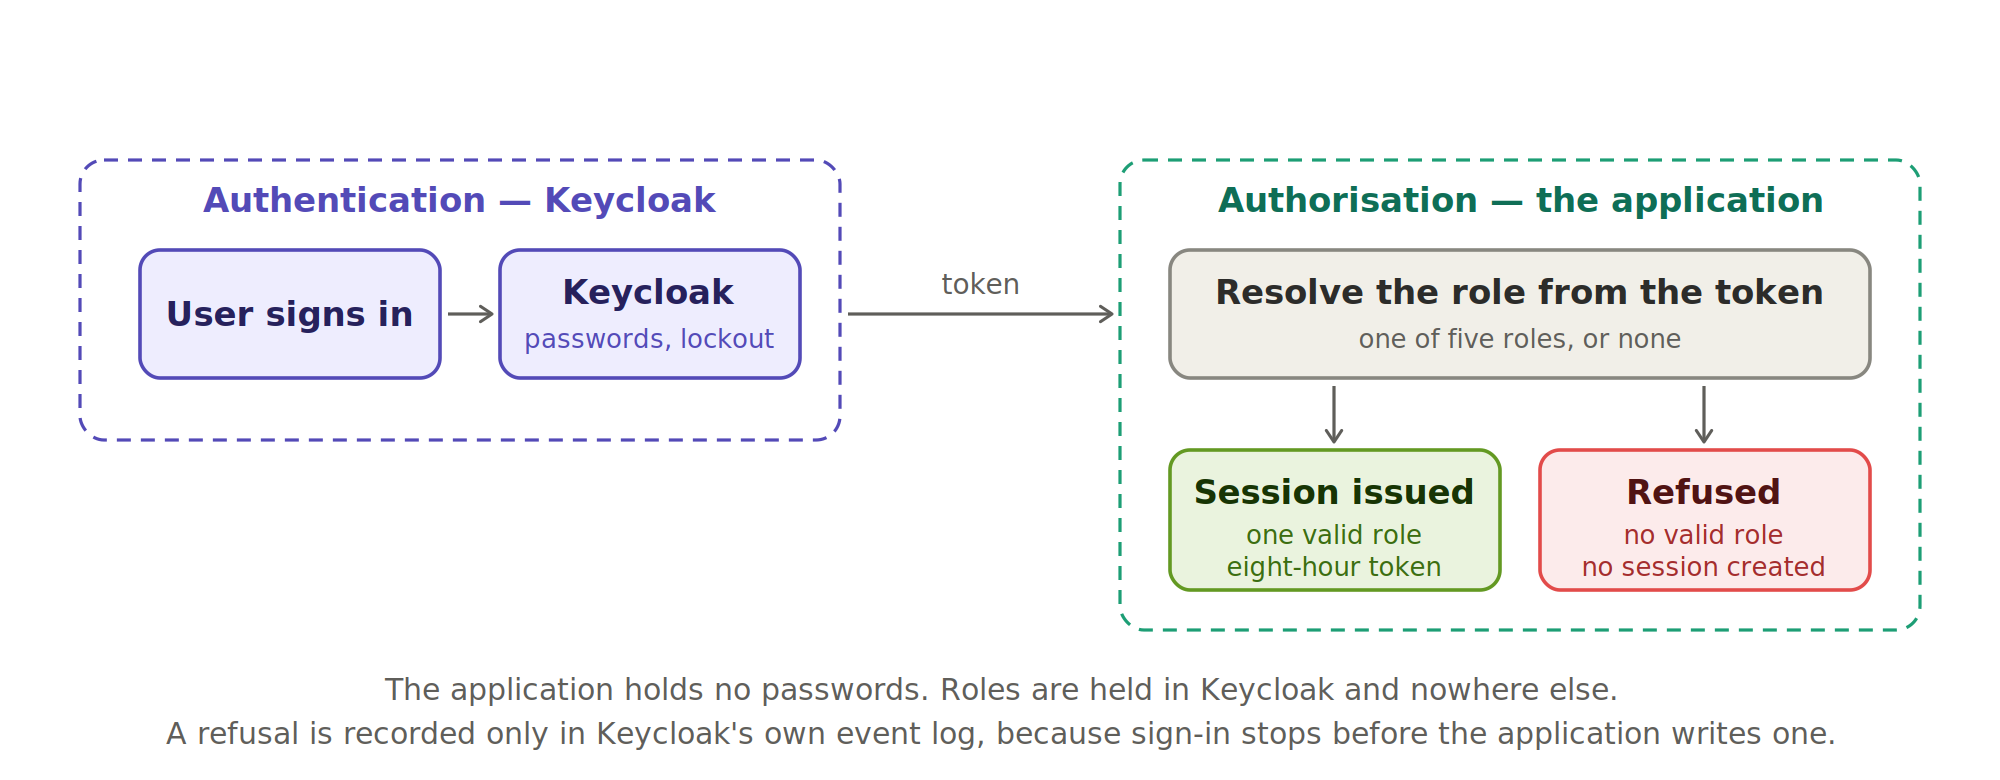
\includegraphics[width=0.95\textwidth]{figs/Figure4-Sign-In-Path.png}
  \caption{The sign-in path. Keycloak checks the password and returns a token carrying the user's identity and role. A token with one valid role gets a session; a token with none is refused.}
  \label{fig:signin-path}
\end{figure}

The server does not keep track of who is signed in. Instead, each user gets a token that proves who they are for eight hours, shortened from the library's default of thirty days. Because there is no server-side list, a token cannot be cancelled early; it stays valid until it expires. Keycloak also keeps its own separate session, timing out after twenty minutes of no activity or eight hours in total. The application adds a further twenty-minute idle timer of its own, with a one-minute warning. This one only runs in the browser: it is a visual timer, not something the server checks. It only catches someone who leaves the tab open and walks away. If the tab is closed instead, even briefly, the timer forgets that time passed and starts again from zero the next time the tab opens. So closing the tab does not stop a different person from opening the browser soon after and landing straight in. The timer also has no effect on the token's own eight-hour lifespan.

Two problems with this design have since been fixed. First, signing out now properly ends both sessions instead of just the application's. Before this fix, the next person on a shared computer could still be signed in as the last user, because only the application's side was cleared. Second, the two systems' timers were brought into line, so neither outlasts the other.

One limitation remains. Because there is no server-side session record, nobody can cancel a token early, and idle time cannot be enforced by the server. A disabled account is no longer part of this problem, since that is now checked directly on every request, described in the next section. But a genuinely stolen token would still work for the rest of its eight hours, since there is still no way to cancel it early.

\subsection{Account Status and AD Federation}

Keycloak originally held its own standalone accounts, created and managed only inside Keycloak itself, separate from any hospital system. During this work, Keycloak was connected to the hospital's own Active Directory through user federation instead (Section \ref{sec:met-tools} describes this decision). Accounts and their enabled or disabled status now come from AD, so a person's access in this system follows the same account AD already manages for them, rather than a separate copy Keycloak held on its own. A background job polls Keycloak every sixty seconds and mirrors its enabled/disabled state into the application's own database; every request checks that mirrored flag, which is what makes the check fast and consistent across every entry point, at the cost of a real but small window, typically under a minute, between a change in Keycloak and the application noticing it.

Access now requires two conditions to hold at once: the account must be enabled in Keycloak, and it must be enabled in the application's own record. The check is centralised in a single function that every entry point calls, so the six surfaces that enforce it (the sign-in check, three separate authorisation helpers used across the application's API routes, the page-level guard that runs on server-rendered navigation, and a client-side watcher that catches cached navigation those other checks do not see) can never disagree with one another. The two conditions are not symmetric. A Keycloak-side disable overrides everything: if Keycloak reports the account disabled, the user is locked out regardless of what the application's own record says, and no administrator can override that from inside the application. An administrator can still enable or disable an account independently through the application's own screen, and that setting is enforced on its own terms whenever Keycloak's side says enabled: an application-side disable still blocks the user even though Keycloak allows them. So the rule is closer to a logical AND than an override: both sides must say enabled, but only one side, Keycloak, can force a lock-out the other side cannot undo. A further condition covers users who disappear from Keycloak or AD entirely rather than being explicitly disabled: such an account is marked disabled in the application with a distinct ``not found'' status, and if that person's account later reappears, they are issued a new account rather than having the old one reactivated, a decision made jointly with the hospital's IT team since silently relinking an old account to a returning identity was judged a greater risk than the inconvenience of starting fresh.

\begin{figure}[H]
  \centering
  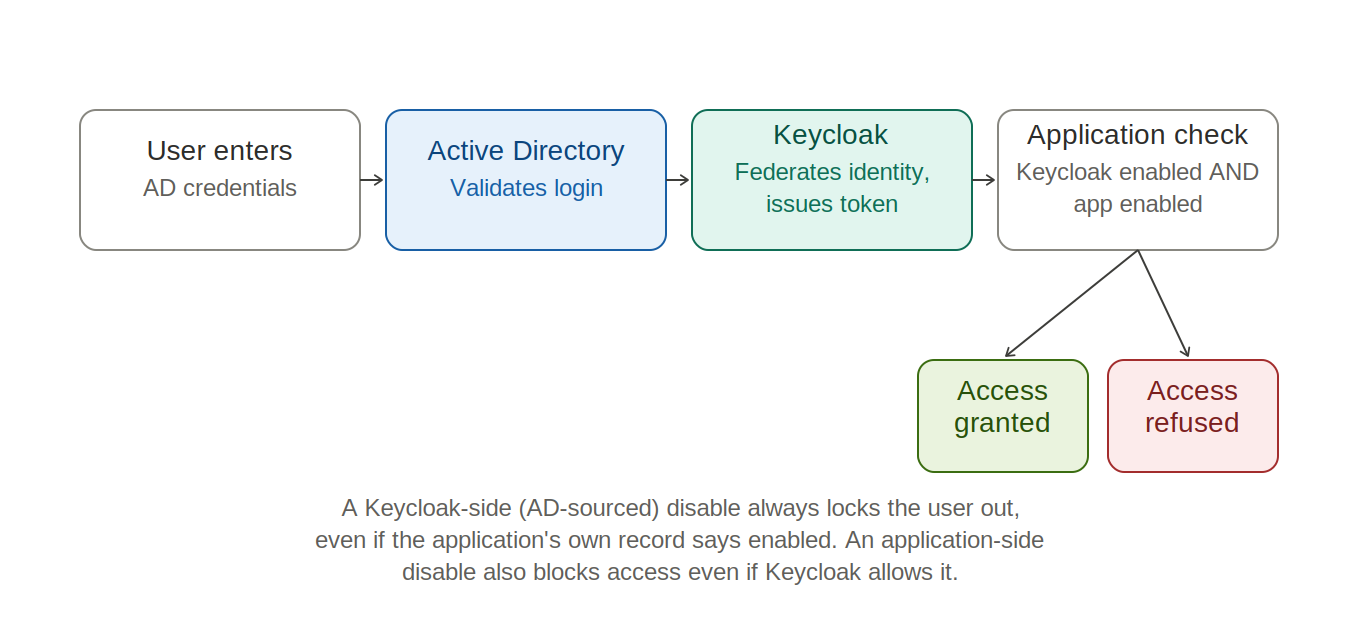
\includegraphics[width=0.95\textwidth]{figs/Figure5-Account-Status-AD-Federation.png}
  \caption{Account status after AD federation. Access requires two conditions to hold at once, checked on every request: the account must be enabled in Keycloak, whose status is itself now sourced from AD through federation, and enabled in the application's own record.}
  \label{fig:account-status}
\end{figure}

This design replaced an earlier approach that never worked. The original plan was a scheduled job: check each user's status against Keycloak on a timer, and disable anyone Keycloak reported as disabled. That job never actually ran, not even once. Its trigger was written to start on a hosting platform this deployment does not use, so nothing ever told it to run, and this was recorded as an open gap.

This is a real improvement over the original job. The original job never ran at all; this one runs reliably every sixty seconds. So the window a disabled account could still be used shrank from indefinite to roughly a minute, though it does not close the gap completely.

Two small limits remain, and neither is a flaw unique to this design. First, the check does not end an already-open browser tab the instant an account is disabled, and a request already in progress at the exact moment the flag flips still completes. This is true of any periodically-synced check. But the user's very next request after that, whether loading a new page or saving a form, is rejected before anything is written, with an ``account disabled'' response, and that refusal is logged. Second, anything the user genuinely did before that point stays correctly recorded; disabling their account part-way through a session does not change what already happened.

The other two background jobs, described in Section \ref{sec:impl-deployment}, are unrelated to account status and were not part of this change; their own outcomes are described there.

The two places used to record changes unevenly. A change made on the application's own screen was written to the audit trail. A change made directly in Keycloak or AD was not, so checking an account's history meant looking in two separate places. This has since been fixed: the same background job that copies a Keycloak-side disable into the application's database now also writes an audit entry at that same moment, so nothing extra is needed to record a Keycloak-side change.

One finding here turned out to matter more than it first looked. The session carries the ID Keycloak issues, but the application's own database uses a different ID for the same people. A check meant to confirm whether a case belonged to a particular doctor was comparing these two different IDs directly, and since they never match, doctors could not open their own cases. This showed up as several separate-looking problems at first: a list showing other people's drafts, a saved draft that opened read-only, and errors when saving. All of them turned out to share the same cause. This was fixed by converting one ID to the other before comparing them.

\section{Access Control Model}
\label{sec:impl-access-model}

Access control in this system combines the two models described in Chapter \ref{chap:lr}. Roles carry the decisions that follow a person's job, attributes carry the decisions that depend on a particular case, and the case's position in the workflow carries the decisions that depend on how far the work has progressed.

Mapped onto the four inputs NIST describes \cite{nist80162}, the model uses three of them. Subject attributes are the user's role, taken from the Keycloak token, and whether their account is active. Object attributes are the identifiers of the doctors assigned to a case and the step that case has reached. The rules are the forty-two action rules described below. Environment conditions are not used: no decision in this system depends on the time of day, the location of the request, or the network it arrives from.

\begin{table}[H]
\centering
\caption{The five roles and what each is responsible for.}
\label{tab:roles}
\begin{tabular}{|p{4.5cm}|p{9.4cm}|}
\hline
\textbf{Role} & \textbf{Responsible for} \\
\hline
Surgeon & Creating a case, entering the clinical description and their own fee \\
\hline
Anaesthetist & Taking an unassigned case from the pool and adding their assessment \\
\hline
Surgical Coordinator & Monitoring progress, and setting case priority \\
\hline
Finance & Building and confirming the cost, submitting the case, recording patient consent, finalising it, reviewing and sending the request to the insurer, and recording the insurer's answer \\
\hline
System Administrator & Managing user accounts, reading the audit trail, viewing all cases and patient data, assigning doctors to cases, and using emergency override powers (releasing a stuck case, removing documents) \\
\hline
\end{tabular}
\end{table}

Forty-two actions are defined across the system, and each has a rule saying which roles may perform it and under what conditions. They fall into four groups: eleven for the case lifecycle, six for finance and the insurer, six for documents and notes, and nineteen for reports, administration and reference data. The rules are kept in a separate document, updated as the code changes. It reached its third version during this work, each version following a round of checking.

The three factors work together, not separately. All three must hold, and if any one fails the action is refused. Take one question: may a surgeon edit this case? Using the role alone, the answer is yes, but that would let any surgeon edit any case. Adding assignment narrows it: yes, if the case is theirs. Adding the step narrows it again: yes, if the case is theirs and it has not yet reached Finance. Only the third answer is correct. The step is the least obvious of the three, because it changes the answer for a user who has done nothing: when the anaesthetist finishes their part, the case moves to Finance, and the surgeon becomes read-only. Figure \ref{fig:three-factors} shows the three factors as they are evaluated for one request.

\begin{figure}[H]
  \centering
  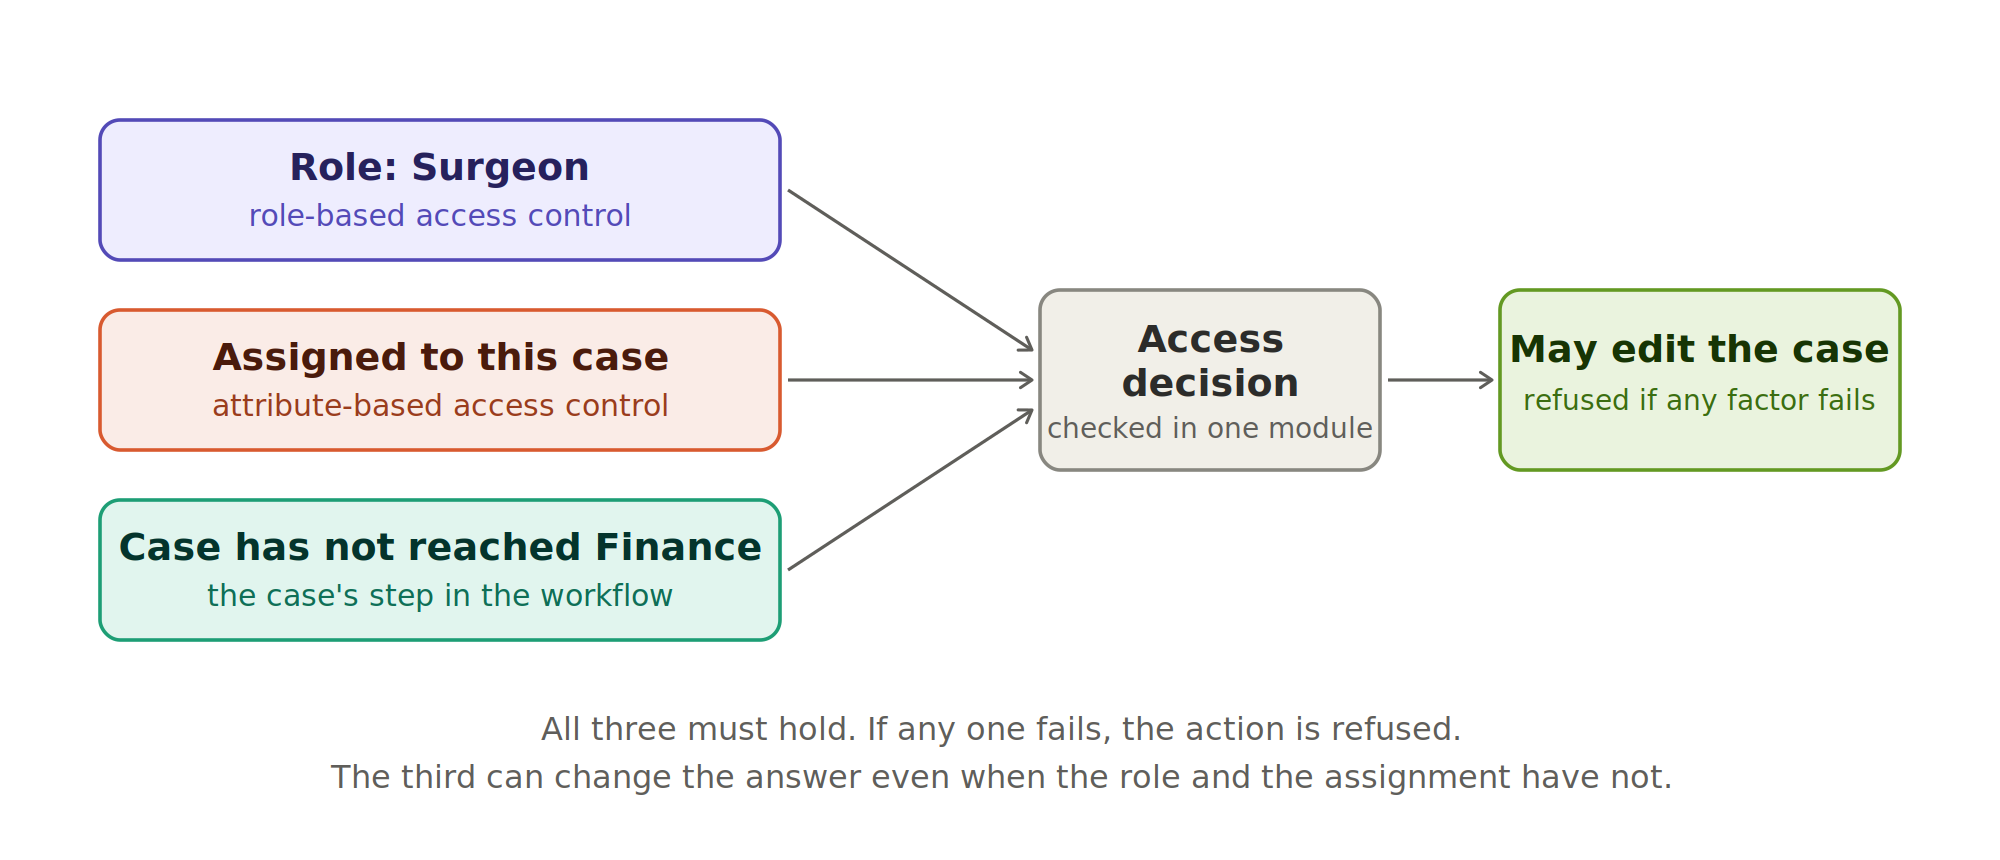
\includegraphics[width=0.95\textwidth]{figs/Figure6-Three-Factors-Decision.png}
  \caption{The three factors evaluated in every access decision. All three must hold; if any one fails, the action is refused.}
  \label{fig:three-factors}
\end{figure}

Underneath these rules is a split the hospital already used on paper. The doctors say what treatment is needed and what their own fee is. Finance builds the final price from that, adding or removing items as the case requires, and commits the hospital to the total. Neither does the other's job: a doctor cannot set what the hospital charges, and Finance does not decide what treatment is given. The case's step is what keeps them apart in software. Without it, a doctor could change a figure after Finance had already settled the price.

The Surgical Coordinator monitors progress and sets case priority; no role holds an edit right over another role's part of a case. The same separation applies to what leaves the hospital; Finance reviews a case before the request is sent, so nothing reaches an insurer without a person having checked it.

Assignment itself needed a rule of its own for the Anaesthetist role. Early on, opening an unassigned case made it the anaesthetist's immediately, with no typing and no saving required, and there was no way to hand it back if it had been opened by mistake. A case is now taken only when the anaesthetist saves or verifies it, and they can release it while it is still a draft. This matters for the same reason the case's step matters elsewhere: an action with a real consequence, becoming responsible for a case, was previously happening as a side effect of merely looking at something.

Access is decided in one place. A single module checks that the user has a session, that their account is active, and that their role is valid. Where the action needs it, the same module also checks that the case is theirs and has reached the right step. Nearly every address in the system calls it. Not every part uses the full check, though: at least eight places ask only whether the role is right, then work out for themselves whether the case belongs to the user, using their own separate copy of that rule rather than the shared one. This has already caused a real problem once, not just a theoretical risk: one of those copies fell out of step with the shared rule and briefly let a surgeon reach a case they should not have been able to see, before it was found and corrected. The other copies currently still agree with the shared rule, kept in sync only by developers remembering to update every copy by hand. Chapter \ref{chap:result} returns to this.

\section{Audit Logging}
\label{sec:impl-audit}

The audit log records every action that changes a case. An entry holds who acted, the role they held at the time, which case was affected, what was done, when, and which part of the system was used. Refused attempts are recorded too, with the reason. The entry does not record the device or the network address, so it can show that an account acted but not which machine was used.

The record is append-only: entries can be added, but never changed or deleted. This is enforced at the database level, through a trigger that rejects any update, delete, or truncate against the table outright, combined with a permission grant that removes the application's own database login's ability to attempt those operations at all. Neither the System Administrator role inside the application, nor a compromised application process using its normal database credentials, can alter a log entry; both are blocked before the operation would even reach the trigger. OWASP recommends exactly this for records that need to be trusted \cite{owasp2021}. It is what makes the log usable as evidence, rather than just something to look things up in.

One honest caveat sits underneath this, distinct from anything reachable through the application: whoever holds the database's own superuser credentials (a different, infrastructure-level actor entirely from any role the application defines) can disable the trigger with an explicit administrative command before modifying rows, then re-enable it. This is not a gap in the design so much as an inherent property of database superuser access generally, and it requires credentials no application role has access to. It happened exactly once, in a local development database, as an authorised, one-off cleanup of test data, carried out as a deliberate and distinct action rather than an ordinary delete, and never applied to the deployed system. Those credentials were handed over to the hospital at the end of the placement; the development team retains no database access on the live system. In short, the immutability guarantee described above is an application-level guarantee, holding against every role the application defines; who controls the database's own infrastructure-level superuser credentials is a separate governance question entirely, answered by who holds server access, not by anything this application can enforce in code.

The log saves a person's exact role at the moment they act, rather than looking it up again later. This fixes a real bug found during the work: Finance and the Coordinator had both been logged under the same generic label, STAFF, so old entries could not show which of the two had actually acted. Saving the exact role at the time also means that if someone's role changes later, old entries still correctly show what their role was back when they acted.

The administration screen presents a second log alongside it, and the two are not the same thing. The audit log records workflow events, as described above. The activity log instead records every successful request that passes the access checks, including the request body itself.

Two problems with this log have since been fixed. First, it had none of the protection the audit log has: rows could be changed or deleted, and no retention period was set. This is now fixed, and the activity log is in fact stricter than the audit log: the audit log's trigger allows one narrow exception (deleting a case correctly clears that entry's case reference), while the activity log has no such exception at all, so its trigger rejects every update, delete, and truncate outright.

Second, because the request body includes patient and clinical fields, those details used to be stored in the clear as a side effect of simply recording traffic. This is also now fixed: those fields are redacted before the row is written, replaced with a fixed marker instead of the real value. One small gap remains: a few fields, such as city, country, and gender, are not yet on that redaction list, so they would still be stored in full if a request happened to carry them. This is recorded as an open item in Section \ref{sec:conc-future}.

Two limits remain. Neither is a fault in the sense of a broken control; the second is a genuine, unresolved inconsistency worth stating precisely. The first is names, and it is more mixed than a single description covers. The audit entry's actor field is a reference to the user, resolved to a display name only when the record is read, so a later change to that person's name changes how every past entry involving them is shown. Separately, many entries also embed a name as literal text inside their own detail, ``Case finalised by John Tan (SURGEON),'' for instance, captured at the moment the action happened, and this text is genuinely frozen: it is written once into the append-only log and the database itself rejects any later change to it. The result is that a single entry can show two different names for the same person if they are renamed in between: the frozen name in the detailed text, and the current name in the actor field next to it, disagreeing with each other on the same row. Users can no longer rename themselves through the application, though an administrator creating or renaming an account, and a later sync that pulls a person's display name from Keycloak on each sign-in, can both still change it this way, so the inconsistency remains reachable. The same current-name behaviour reaches insurer emails, printed forms and the coordinator export, so a rename can also affect documents that have already left the hospital, independent of the log itself. The second limit is who may read the log. Administrators open it through the administration screen built as part of this work, and their own actions appear in both logs, so they can see what has been recorded about them. Separating those two responsibilities would mean redesigning who can read what, not fixing a fault.

Four things are not written down. A refusal that means only ``not yet'' (submitting a case before it is ready, or deleting one that has moved past draft) comes from the workflow rather than from a permission check, and only permission refusals are written down. A request for a case that does not exist is refused silently. A refused sign-in is recorded nowhere in the application, because sign-in stops before anything is written, so those attempts exist only in Keycloak's log. And nothing at all can be written when the database itself is down.

Nothing checks the log as it fills, and nobody reviews it on a schedule. Refused attempts are written down correctly, but no one is told, so twenty attempts in a row would sit in the table until somebody happened to open it. OWASP renamed this category in 2025 to include alerting for that reason \cite{owasp2025}. Both are recorded in Section \ref{sec:conc-future}: the software that would raise an alert, and the hospital routine that would review the records.

\section{Deployment}
\label{sec:impl-deployment}

My teammate deployed the application, and the hospital's IT department provided the server. What follows is about the security of that environment: what I found in its configuration, what was corrected, and what is still open.

The system runs on a Windows server the hospital owns, reachable only from inside the hospital. Four programs run on it side by side: the application, the database, Keycloak, and the FHIR server. None of them can be reached from the internet.

Among the four, the database and the FHIR server are the most locked down: only the machine itself can reach them, nothing else. Keycloak is the one deliberate exception. It can be reached from elsewhere on the hospital's internal network, though still never from the internet, because a person's browser needs to talk to Keycloak directly during sign-in.

Patient data is read from the hospital's own system, with limited read-only access granted by the IT department. This deployment does not own or hold the primary patient record; ANZER remains the single source of truth for that data, as Section \ref{sec:met-tools} states.

That said, patient information can still end up inside this system's own storage in one place. As Section \ref{sec:impl-audit} describes, the activity log records the body of every successful request, and some of those requests carry patient identifiers and clinical detail. That information used to be stored as-is, as a side effect of logging traffic. It is now redacted before the row is written, though a small number of fields are not yet covered, recorded as an open item in Section \ref{sec:conc-future}.

The application has a shortcut for developers: skip sign-in, pick a role, no password. It is useful on a laptop and dangerous on a server. The template that people copy when setting up a new server had that shortcut switched on, so anyone following it would have built a server that anyone could walk into. This was fixed twice. The template now has it switched off, and the application refuses to start if the shortcut is on in production.

The browser-facing connection now runs over HTTPS. Two internal connections remain unencrypted: Keycloak to the application, and Keycloak to Active Directory, so credentials and status information passing over those two links still cross the network in the clear. Keycloak also cannot leave its development mode until its own connections are encrypted. Whether the database's disk is encrypted has not been confirmed either way. On a Windows server, that would mean turning on BitLocker, which is a setting on the server itself, not something this application configures, so it is a decision for the server administrator to make.

The four containers are third-party software, so rather than assume they were safe I scanned them, and Chapter \ref{chap:result} reports what that found. One problem was found without a scanner. Keycloak had not been told where to keep its accounts, so it had defaulted to H2, the lightweight, file-based database built into Keycloak itself, meant only for local testing and explicitly not recommended by its makers for a real deployment. H2 stores its data as a single file inside the Keycloak container rather than as a separate, durable service, so losing that container would have meant losing every account outright, and the file could not be backed up without shutting Keycloak down first to release it. Keycloak was reconfigured to use the PostgreSQL database already running alongside it instead, in a separate schema with its own restricted login, so accounts now live in the same durable, backed-up database as the rest of the system rather than a throwaway file tied to one container's lifetime.

Three background jobs existed at the time this was written. One was meant to disable an account when Keycloak said it should be disabled, described in Section \ref{sec:impl-iam}. Another was meant to warn staff when a case was taking too long. A third was meant to close cases automatically once they passed a deadline.

None of the three ever ran, and all three failed for the same reason: their schedule was written in a format meant for a specific cloud hosting service, one this project does not use. The hospital's own server had no way to read that format, so nothing ever told these jobs to start.

One of the three also had a second, separate way it was supposed to run, triggered from the browser whenever the application was open. This did not work either: it used the wrong technical method to make the request, so the server rejected it immediately, before the job itself ever ran.

Each of the three broken jobs has since taken a different path. The account-disable job was not fixed directly; it was replaced entirely by the periodic dual-check design described in Section \ref{sec:impl-iam}. The deadline-closure job was removed outright, a deliberate decision rather than a fix: it used to close cases after a flat 30-day window, unrelated to the SLA tiers described below, and before deletion, a database check confirmed it had never actually closed a single case in the system's history. The slow-case warning job was kept and given a real trigger, but not the one originally planned: instead of an OS-level scheduler like Windows Task Scheduler, it now runs on a timer inside the application itself, firing every 15 minutes while the application is running, a real fix, but a weaker guarantee than an OS-level schedule, since this timer stops if the application process stops.

The rule the slow-case warning job checks against was also revised after this was first written. Cases originally fell into two service-level categories, adjustable from a settings screen. This was changed to three fixed categories: Emergency (1 hour), Urgent (8 hours), and Routine (48 hours). Each number is a threshold, the number of hours a case may wait before it counts as overdue for that category, read from a database-backed configuration rather than the earlier hardcoded pair. The permission to change these three thresholds was built for the Surgical Coordinator and System Administrator roles, with validation, a database write, and its own audit entry, and this was tested working.

This is a different thing from changing an individual case's own category, which is a separate, everyday action the Coordinator still performs normally, described in Section \ref{sec:impl-access-model}; what is disabled here is only the ability to edit the three threshold numbers themselves. This ability to change the thresholds is not usable today. Both the screen that edits them and the route behind it are switched off, deliberately, behind a single flag. This was done after testing found two real bugs in the editor: a saved total that was written but never read anywhere, and a dashboard countdown that used a separate table the editor did not update. Rather than ship a partially working editor, both the screen and the route were locked pending a decision. The route also refuses every request outright, no matter who is asking, so a disabled feature can never be mistaken in the logs for someone being refused because of their role.

Reading the current thresholds still works for everyone. Only changing them is switched off. So in practice, the thresholds are fixed for every role today, though not because that was the design. The ability to adjust them exists, and has been built and tested; it is simply waiting on that flag to be turned on.

This job does not wait until the deadline to raise a warning. Instead, it raises its warning in stages as a case approaches each threshold. The warning itself only shows up inside the application, as a status or a flag; it is not sent out as an email.

These three tiers apply only to this warning job. They do not apply to the separate deadline-closure feature described earlier. That feature used its own unrelated rule, a flat 30-day window, and was removed entirely rather than being connected to this newer, tiered system.
